\documentclass{beamer}
\usepackage[utf8]{inputenc}
\usepackage{graphicx, epsfig}
\usepackage{amsmath,mathrsfs,amsfonts,amssymb}
\usepackage{floatflt}
\usepackage{epic,ecltree}
\usepackage{mathtext}
\usepackage{fancybox}
\usepackage{fancyhdr}
\usepackage{multirow}
\usepackage{enumerate}
\usepackage{epstopdf}
\usepackage{multicol}
\usepackage{algorithm}
\usepackage[noend]{algorithmic}
\usepackage{tikz}
\usepackage{blindtext}
\usepackage{multido}
\usetheme{default}%{Singapore}%{Warsaw}%{Warsaw}%{Darmstadt}
\usecolortheme{default}

\setbeamerfont{title}{size=\Huge}
\setbeamertemplate{footline}[frame number]{}

\setbeamertemplate{section in toc}[sections numbered]

\makeatletter
\newcommand\HUGE{\@setfontsize\Huge{35}{40}}
\makeatother    

\setbeamerfont{title}{size=\HUGE}
\beamertemplatenavigationsymbolsempty

\usetikzlibrary{arrows,shapes,positioning,shadows,trees}

\newcommand\myfootnote[1]{%
  \vspace{-0.5cm}%
  \tikz[remember picture,overlay]
  \draw (current page.south west) +(1in + \oddsidemargin,0.5em)
  node[anchor=south west,inner sep=0pt]{\parbox{\textwidth}{%
      \rlap{\rule{10em}{0.4pt}}\raggedright\scriptsize \textit{#1}}};}

\newcommand\myfootnotewithlink[2]{%
  \vspace{-0.5cm}%
  \tikz[remember picture,overlay]
  \draw (current page.south west) +(1in + \oddsidemargin,0.5em)
  node[anchor=south west,inner sep=0pt]{\parbox{\textwidth}{%
      \rlap{\rule{10em}{0.4pt}}\raggedright\scriptsize\href{#1}{\textit{#2}}}};}

\AtBeginSection[]
      {
      	\begin{frame}{Outline}
      		\tableofcontents[currentsection]
      	\end{frame}
      }
      \AtBeginSubsection[]{
      	\begin{frame}{Outline}
      		\tableofcontents[currentsection,currentsubsection]
      	\end{frame}
}

\newcounter{noscounter} % Используется для nextonslide команды (обнуляется только на новом слайде)
\newcounter{pcounter} % Используется для pause команды (обнуляется после использования eqpause)
\newcounter{diffcounter} % Считает количество pause после формулы

\newcommand{\nextonslide}[1]{%
  \stepcounter{noscounter}% Прибавляем счетчик nextonslide
  \stepcounter{pcounter}% Прибавляем счетчик pause
  \stepcounter{diffcounter}% Прибавляем счетчик diffcounter
  \onslide<\value{noscounter}->{#1}% Отображаем аргумент в скобках на слайде с номером noscounter
}
\newcommand{\resetonslide}{%
    \setcounter{noscounter}{1}% Сбрасываем счетчик nextonslide
    \setcounter{pcounter}{1}% Сбрасываем счетчик pause
    \setcounter{diffcounter}{0}% Сбрасываем счетчик diffcounter
}

\newcommand{\eqpause}{%
  \multido{\i=1+1}{\value{pcounter}}{\pause}% Повторяем pcounter раз команду pause
  \stepcounter{noscounter}% Прибавляем счетчик nextonslide
  \setcounter{pcounter}{1}% Сбрасываем счетчик pause
}

\newcommand{\eqpausediff}{% Вспомогательная команда, запускается автоматически после формул
  \multido{\i=1+1}{\value{diffcounter}}{\pause}% Повторяем diffcounter раз команду pause
  \addtocounter{pcounter}{-\value{diffcounter}}% Вычитаем из pcounter количество сделанных pause
  \setcounter{diffcounter}{0}% Сбрасываем счетчик diffcounter
}

\newcommand\AtEndBoth[2]{% Применяем команду к multline и multline*
  \AtEndEnvironment{#1}{#2}%
  \AtEndEnvironment{#1*}{#2}%
}

\AtEndBoth{align}{\eqpausediff}
\AtEndBoth{equation}{\eqpausediff}
\AtEndBoth{multline}{\eqpausediff}

\addtobeamertemplate{frametitle}{\resetonslide}{}% На каждом слайде сбрасываем счетчики

% latin bold lower
\newcommand{\ba}{\mathbf{a}} 
\newcommand{\bc}{\mathbf{c}} 
\newcommand{\be}{\mathbf{e}} 
\newcommand{\bff}{\mathbf{f}} % \bf - for bold type
\newcommand{\bg}{\mathbf{g}} 
\newcommand{\bh}{\mathbf{h}} 
\newcommand{\bp}{\mathbf{p}} 
\newcommand{\bq}{\mathbf{q}} 
\newcommand{\bt}{\mathbf{t}} 
\newcommand{\bs}{\mathbf{s}} 
\newcommand{\bu}{\mathbf{u}} 
\newcommand{\bv}{\mathbf{v}} 
\newcommand{\bw}{\mathbf{w}} 
\newcommand{\bx}{\mathbf{x}} 
\newcommand{\by}{\mathbf{y}} 
\newcommand{\bz}{\mathbf{z}} 

% latin bold upper
\newcommand{\bA}{\mathbf{A}} 
\newcommand{\bB}{\mathbf{B}} 
\newcommand{\bC}{\mathbf{C}} 
\newcommand{\bG}{\mathbf{G}} 
\newcommand{\bI}{\mathbf{I}} 
\newcommand{\bJ}{\mathbf{J}} 
\newcommand{\bL}{\mathbf{L}} 
\newcommand{\bM}{\mathbf{M}} 
\newcommand{\bP}{\mathbf{P}}
\newcommand{\bQ}{\mathbf{Q}} 
\newcommand{\bR}{\mathbf{R}} 
\newcommand{\bT}{\mathbf{T}} 
\newcommand{\bU}{\mathbf{U}} 
\newcommand{\bV}{\mathbf{V}} 
\newcommand{\bW}{\mathbf{W}} 
\newcommand{\bX}{\mathbf{X}} 
\newcommand{\bY}{\mathbf{Y}} 
\newcommand{\bZ}{\mathbf{Z}} 

% latin cal upper
\newcommand{\cF}{\mathcal{F}} 
\newcommand{\cG}{\mathcal{G}} 
\newcommand{\cI}{\mathcal{I}} 
\newcommand{\cL}{\mathcal{L}} 
\newcommand{\cM}{\mathcal{M}} 
\newcommand{\cN}{\mathcal{N}} 
\newcommand{\cP}{\mathcal{P}} 
\newcommand{\cS}{\mathcal{S}} 
\newcommand{\cT}{\mathcal{T}} 
\newcommand{\cW}{\mathcal{W}} 
\newcommand{\cX}{\mathcal{X}} 
\newcommand{\cZ}{\mathcal{Z}} 

% latin bb upper
\newcommand{\bbE}{\mathbb{E}} 
\newcommand{\bbI}{\mathbb{I}} 
\newcommand{\bbP}{\mathbb{P}} 
\newcommand{\bbR}{\mathbb{R}} 

% greek bold lower
\newcommand{\bepsilon}{\boldsymbol{\epsilon}} 
\newcommand{\btheta}{\boldsymbol{\theta}} 
\newcommand{\blambda}{\boldsymbol{\lambda}} 
\newcommand{\bpi}{\boldsymbol{\pi}} 
\newcommand{\bmu}{\boldsymbol{\mu}} 
\newcommand{\bsigma}{\boldsymbol{\sigma}} 
\newcommand{\bphi}{\boldsymbol{\phi}} 

% greek bold upper
\newcommand{\bSigma}{\boldsymbol{\Sigma}} 

\DeclareMathOperator*{\argmin}{arg\,min}
\DeclareMathOperator*{\argmax}{arg\,max}
\newcommand{\createdgmtitle}[1]{\title[\hbox to 56mm{Deep Generative Models  \hfill\insertframenumber\,/\,\inserttotalframenumber}]
	{\vspace{1cm} \\ \textbf{Deep Generative Models} \\ {\Huge Lecture #1}}
	\author{Roman Isachenko}
	\institute{
		Moscow Institute of Physics and Technology \\
		Yandex School of Data Analysis
	}
	\date{2025, Autumn}
}
\createdgmtitle{3}

%--------------------------------------------------------------------------------
\begin{document}
%--------------------------------------------------------------------------------
\begin{frame}[noframenumbering,plain]
	\titlepage
	\resetonslide
\end{frame}
%=======
\begin{frame}{Recap of Previous Lecture}
    \myfootnotewithlink{https://arxiv.org/abs/1605.08803}{Dinh L., Sohl-Dickstein J., Bengio S. Density Estimation Using Real NVP, 2016} 
	\begin{block}{Jacobian Matrix}
		Given a differentiable function $\bff: \bbR^m \rightarrow \bbR^m$,
		\[
		\bz = \bff(\bx), \quad 
		\bJ =  \frac{\partial \bz}{\partial \bx} =
		\begin{pmatrix}
			\frac{\partial z_1}{\partial x_1} & \dots & \frac{\partial z_1}{\partial x_m} \\
			\vdots & \ddots & \vdots \\ 
			\frac{\partial z_m}{\partial x_1} & \dots & \frac{\partial z_m}{\partial x_m}
		\end{pmatrix} \in \bbR^{m \times m}
		\]
		\vspace{-0.3cm}
	\end{block}
	\begin{block}{Change of Variables Theorem (CoV)}
		Let $\bx$ be a random variable with density $p(\bx)$, and $\bff: \bbR^m \rightarrow \bbR^m$ a differentiable invertible mapping. If $\bz = \bff(\bx)$ and $\bx = \bff^{-1}(\bz) = \bg(\bz)$, then
		\vspace{-0.3cm}
		\begin{align*}
			p(\bx) &= p(\bz) |\det(\bJ_\bff)| = p(\bz) \left|\det \left(  \frac{\partial \bz}{\partial \bx} \right) \right| = p(\bff(\bx)) \left|\det \left(  \frac{\partial \bff(\bx)}{\partial \bx} \right) \right| \\
			p(\bz) &= p(\bx) |\det(\bJ_\bg)|= p(\bx) \left|\det \left(  \frac{\partial \bx}{\partial \bz} \right) \right| = p(\bg(\bz)) \left|\det \left(  \frac{\partial \bg(\bz)}{\partial \bz} \right) \right|.
		\end{align*}
	\end{block}
\end{frame}
%=======
\begin{frame}{Recap of Previous Lecture}
    \myfootnotewithlink{https://arxiv.org/abs/1605.08803}{Dinh L., Sohl-Dickstein J., Bengio S. Density Estimation Using Real NVP, 2016} 
	\begin{block}{Definition}
		A normalizing flow is a \textit{differentiable, invertible} transformation that maps data $\bx$ to noise $\bz$. 
	\end{block}
	\vspace{-0.1cm}
	\begin{figure}
		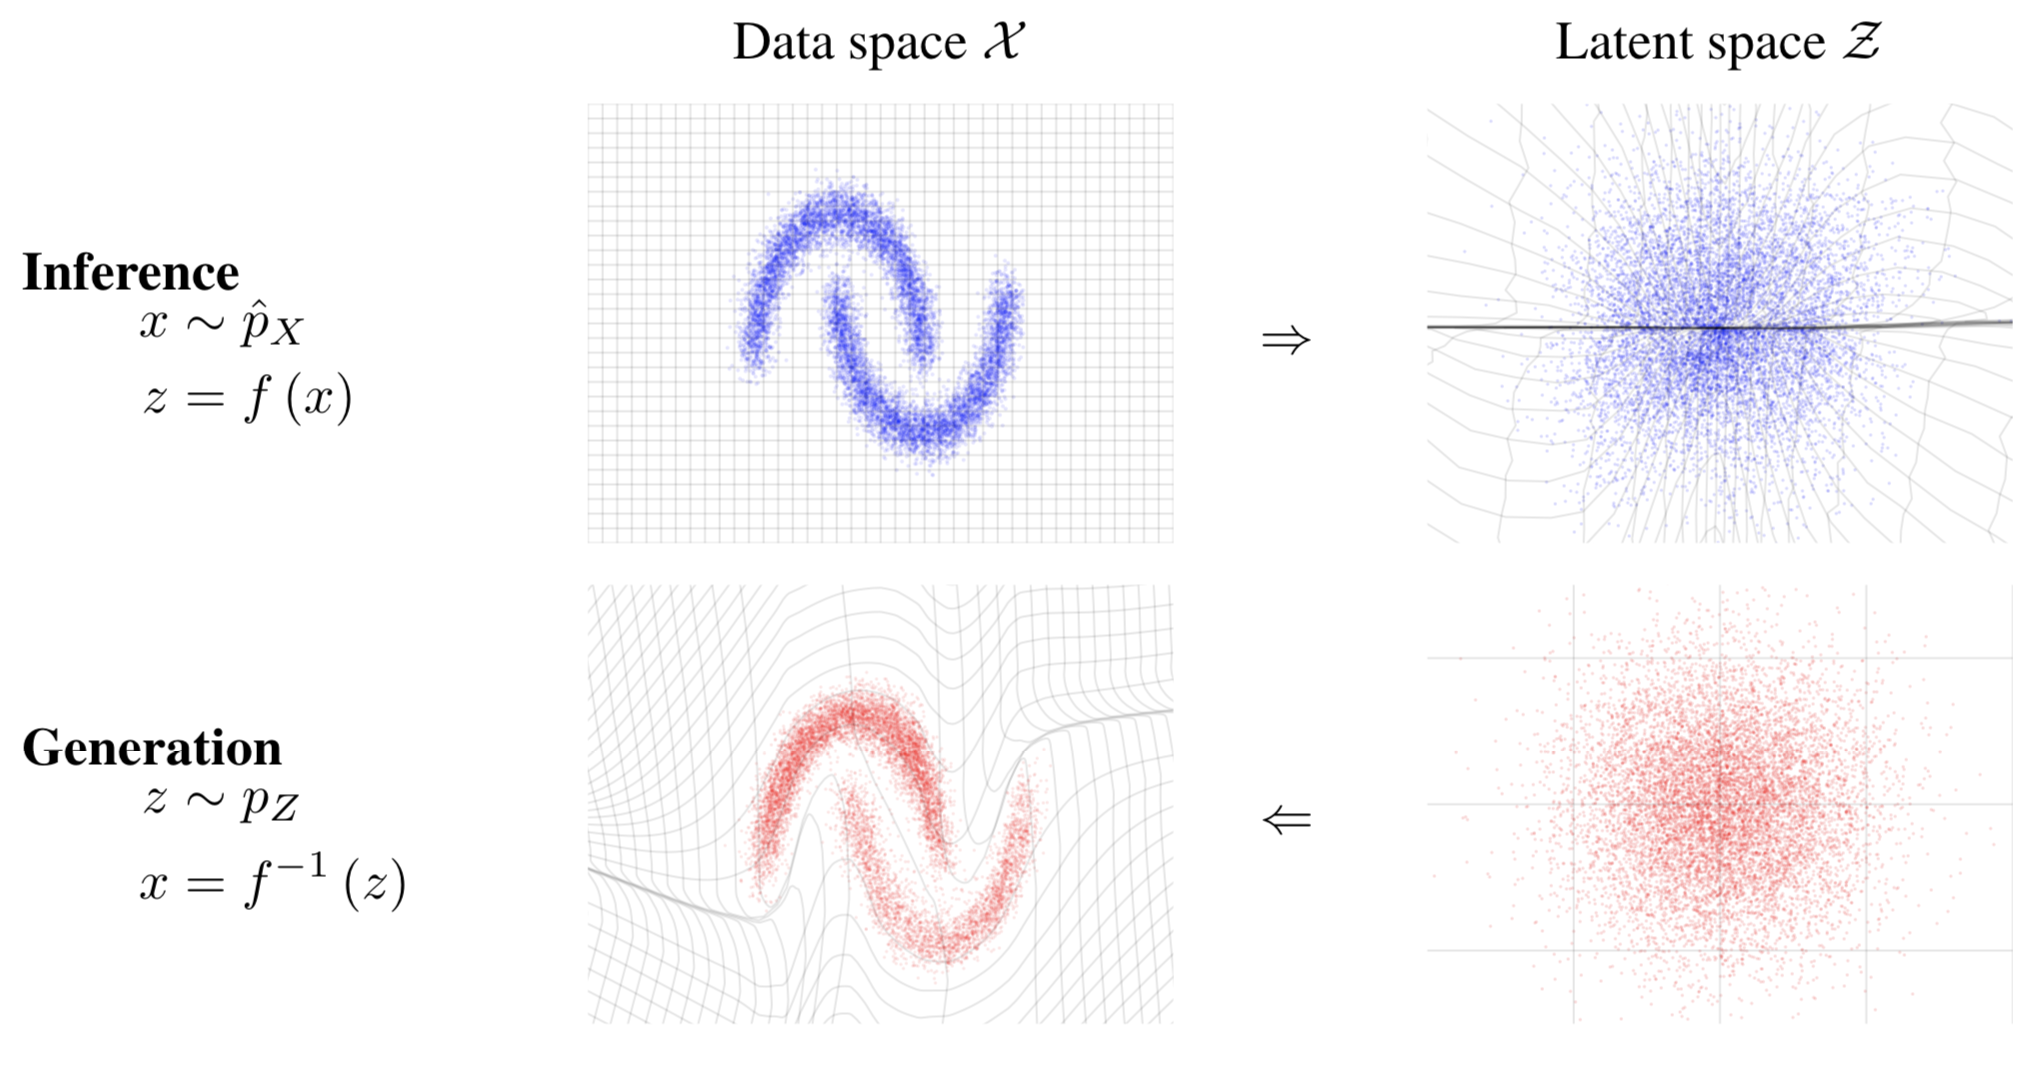
\includegraphics[width=0.85\linewidth]{figs/flows_how2}
	\end{figure}
	\vspace{-0.5cm}
	\begin{block}{Log-Likelihood}
		\vspace{-0.5cm}
		\[
			\log p(\bx | \btheta) = \log p(\bff_K \circ \cdots \circ \bff_1(\bx)) + \sum_{k=1}^K\log |\det (\bJ_{\bff_k})|
		\]
	\end{block}
\end{frame}
%=======
\begin{frame}{Recap of Previous Lecture}
    \myfootnote{\href{https://arxiv.org/abs/1807.03039}{Kingma D. P., et al. Glow: Generative Flow With Invertible 1x1 Convolutions, 2018}  \\
	\href{https://arxiv.org/abs/1901.11137}{Hoogeboom E., et al. Emerging Convolutions for Generative Normalizing Flows, 2019}
	}
	\vspace{-0.5cm}
	\begin{block}{Flow Log-Likelihood}
		\vspace{-0.3cm}
		\[
			\log p(\bx|\btheta) = \log p(\bff_{\btheta}(\bx)) + \log |\det (\bJ_\bff)|
		\]
		\vspace{-0.5cm}
	\end{block}
	One significant challenge is efficiently computing the Jacobian determinant.
	\begin{block}{Linear Flows}	
		\vspace{-0.2cm}
		\[
			\bz = \bff_{\btheta}(\bx) = \bW \bx, \quad \bW \in \bbR^{m \times m}, \quad \btheta = \bW, \quad \bJ_\bff = \bW^T
		\]
	\end{block}
	\vspace{-0.3cm}
	\begin{itemize}
		\item LU Decomposition:
		\[
			\bW = \bP \bL \bU.
		\]
		\item QR Decomposition:
		\[
			\bW = \bQ \bR.
		\]
	\end{itemize}
	Decomposition is performed only once during initialization. Then the decomposed matrices ($\bP, \bL, \bU$ or $\bQ, \bR$) are optimized.
\end{frame}
%=======
\begin{frame}{Recap of Previous Lecture}
    \myfootnotewithlink{https://arxiv.org/abs/1705.07057}{Papamakarios G., Pavlakou T., Murray I. Masked Autoregressive Flow for Density Estimation, 2017} 
	Consider an autoregressive model:
	\vspace{-0.3cm}
	{\small
		\[
		p(\bx | \btheta) = \prod_{j=1}^m p(x_j | \bx_{1:j - 1}, \btheta), \quad
		p(x_j | \bx_{1:j - 1}, \btheta) = \cN \left(\mu_{j, \btheta}(\bx_{1:j-1}), \sigma^2_{j, \btheta} (\bx_{1:j-1})\right).
		\]
	}
	\vspace{-0.5cm}
	\begin{block}{Gaussian Autoregressive Normalizing Flow}
		\vspace{-0.5cm}
		\begin{align*}
			\bx &= \bg_{\btheta}(\bz) \quad \Rightarrow \quad {\color{violet} x_j} = \sigma_{j, \btheta} ({\color{violet} \bx_{1:j-1}}) \cdot {\color{teal} z_j} + \mu_{j, \btheta}({\color{violet} \bx_{1:j-1}}). \\
			\bz &= \bff_{\btheta}(\bx) \quad \Rightarrow \quad {\color{teal} z_j} = \left({\color{violet}x_j} - \mu_{j, \btheta}({\color{violet}\bx_{1:j-1}}) \right) \cdot \frac{1}{ \sigma_{j, \btheta} ({\color{violet}\bx_{1:j-1}})}.
		\end{align*}
		\vspace{-0.5cm}
	\end{block}
	\begin{itemize}
		\item This transformation is both \textbf{invertible} and \textbf{differentiable}, mapping $p(\bz)$ to $p(\bx | \btheta)$.
		\item The Jacobian matrix for this transformation is triangular.
	\end{itemize}
	The generative function $\bg_{\btheta}(\bz)$ is \textbf{sequential}, while the inference function $\bff_{\btheta}(\bx)$ is \textbf{not sequential}.
\end{frame}
%=======
\begin{frame}{Recap of Previous Lecture}
    \myfootnotewithlink{https://arxiv.org/abs/1605.08803}{Dinh L., Sohl-Dickstein J., Bengio S. Density Estimation Using Real NVP, 2016} 

	Let us partition $\bx$ and $\bz$ into two groups: 
	\[
		\bx = [\bx_1, \bx_2] = [\bx_{1:d}, \bx_{d+1:m}]; \quad \bz = [\bz_1, \bz_2] = [\bz_{1:d}, \bz_{d+1:m}].
	\]
	\vspace{-0.7cm}
	\begin{block}{Coupling Layer}
		\vspace{-0.7cm}
		\[
			\begin{cases} {\color{violet}\bx_1} = {\color{teal}\bz_1}; \\ {\color{violet}\bx_2} = {\color{teal}\bz_2} \odot \bsigma_{\btheta}({\color{teal}\bz_1}) + \bmu_{\btheta}({\color{teal}\bz_1}).\end{cases}  
			\begin{cases} {\color{teal}\bz_1} ={\color{violet} \bx_1}; \\ {\color{teal}\bz_2} = \left({\color{violet}\bx_2} - \bmu_{\btheta}({\color{violet}\bx_1}) \right) \odot \frac{1}{\bsigma_{\btheta}({\color{violet}\bx_1})}.\end{cases}
		\]
		Both density estimation and sampling require just a single pass!
	\end{block}
	\begin{block}{Jacobian}
		\vspace{-0.3cm}
		\[
			\det \left( \frac{\partial \bz}{\partial \bx} \right) = \det 
			\begin{pmatrix}
				\bI_d & 0_{d \times (m - d)} \\
				\frac{\partial \bz_2}{\partial \bx_1} & \frac{\partial \bz_2}{\partial \bx_2}
			\end{pmatrix} = \prod_{j=1}^{m - d} \frac{1}{\sigma_{j, \btheta}(\bx_1)}.
		\]
	\end{block}
	A coupling layer is a special instance of an gaussian autoregressive normalizing flow.
\end{frame}
%=======
\begin{frame}{Outline}
    \tableofcontents
\end{frame}
%=======
\section{Latent Variable Models (LVM)}
%=======
\begin{frame}{Bayesian Framework}
	\begin{block}{Bayes' Theorem}
		\vspace{-0.3cm}
		\[
			p(\btheta| \bx) = \frac{p(\bx | \btheta) p(\btheta)}{p(\bx)} = \frac{p(\bx | \btheta) p(\btheta)}{\int p(\bx | \btheta) p(\btheta) d \btheta} 
		\]
		\vspace{-0.3cm}
		\begin{itemize}
			\item $\bx$: observed variables; 
			\item $\btheta$: unknown latent variables/parameters;
			\item $p(\bx | \btheta)$: likelihood;
			\item $p(\bx) = \int p(\bx | \btheta) p(\btheta) d\btheta$: evidence;
			\item $p(\btheta)$: prior distribution;
			\item $p(\btheta| \bx)$: posterior distribution.
		\end{itemize}
	\end{block}
    \eqpause
	\begin{block}{Interpretation}
		\begin{itemize}
			\item We begin with unknown variables $\btheta$ and a prior belief $p(\btheta)$.
			\item Once data $\bx$ is observed, the posterior $p(\btheta| \bx)$ incorporates both prior beliefs and evidence from the data.
		\end{itemize} 
	\end{block}
\end{frame}
%=======
\begin{frame}{Bayesian Framework}
	Consider the case where the unobserved variables $\btheta$ are model parameters (i.e., $\btheta$ are random variables).
	\begin{itemize}
		\item $\bX = \{\bx_i\}_{i=1}^n$: observed samples;
		\item $p(\btheta)$: prior distribution.
	\end{itemize}
    \eqpause
	\begin{block}{Posterior Distribution}
		\[
			p(\btheta | \bX) = \frac{p(\bX | \btheta) p(\btheta)}{p(\bX)} = \frac{p(\bX | \btheta) p(\btheta)}{\int p(\bX | \btheta) p(\btheta) d \btheta} 
		\]
		\vspace{-0.2cm}
	\end{block}
    \eqpause
	If the evidence $p(\bX)$ is intractable (due to high-dimensional integration), the posterior cannot be computed exactly.
    \eqpause
    \begin{block}{Maximum a Posteriori (MAP) Estimation}
	    \vspace{-0.2cm}
	    \[
	        \btheta^* = \argmax_{\btheta} p(\btheta | \bX) = \argmax_{\btheta} (\log p(\bX | \btheta) + \log p(\btheta))
	    \]
    \end{block}
\end{frame}
%=======
\begin{frame}{Latent Variable Models (LVM)}
	\begin{block}{Maximum Likelihood Extimation (MLE) Problem}
		\vspace{-0.7cm}
		\[
		\btheta^* = \argmax_{\btheta} p(\bX | \btheta) = \argmax_{\btheta} \prod_{i=1}^n p(\bx_i | \btheta) = \argmax_{\btheta} \sum_{i=1}^n \log p(\bx_i | \btheta).
		\]
		\vspace{-0.5cm}
	\end{block}
    \eqpause
	The distribution $p(\bx | \btheta)$ can be highly complex and often intractable (just like the true data distribution $\pi(\bx)$).
    \eqpause
	\begin{block}{Extended Probabilistic Model}
		Introduce a latent variable $\bz$ for each observed sample $\bx$:
		\[
			p(\bx, \bz | \btheta) = p(\bx | \bz, \btheta) p(\bz); \quad 
		\log p(\bx, \bz | \btheta) = \log p(\bx | \bz, \btheta) + \log p(\bz).
		\]
		\[
			\nextonslide{p(\bx | \btheta) = \int p(\bx, \bz | \btheta) d\bz = \int p(\bx | \bz, \btheta) p(\bz) d\bz.}
		\]
	\end{block}
    \eqpause
	\vspace{-0.3cm}
	\begin{block}{Motivation}
		Both $p(\bx | \bz, \btheta)$ and $p(\bz)$ are usually much simpler than $p(\bx | \btheta)$.
	\end{block}
\end{frame}
%=======
\begin{frame}{Latent Variable Models (LVM)}
    \myfootnote{Bishop\,C. Pattern Recognition and Machine Learning, 2006}
	\[
		\log p(\bx | \btheta) = \log \int p(\bx | \bz, \btheta) p(\bz) d\bz \rightarrow \max_{\btheta}
	\]
    \eqpause
	\vspace{-0.6cm}
	\begin{block}{Examples}
		\begin{minipage}[t]{0.45\columnwidth}
			\textit{Mixture of Gaussians} \\
			\vspace{-0.5cm}
			\begin{figure}
				\centering
				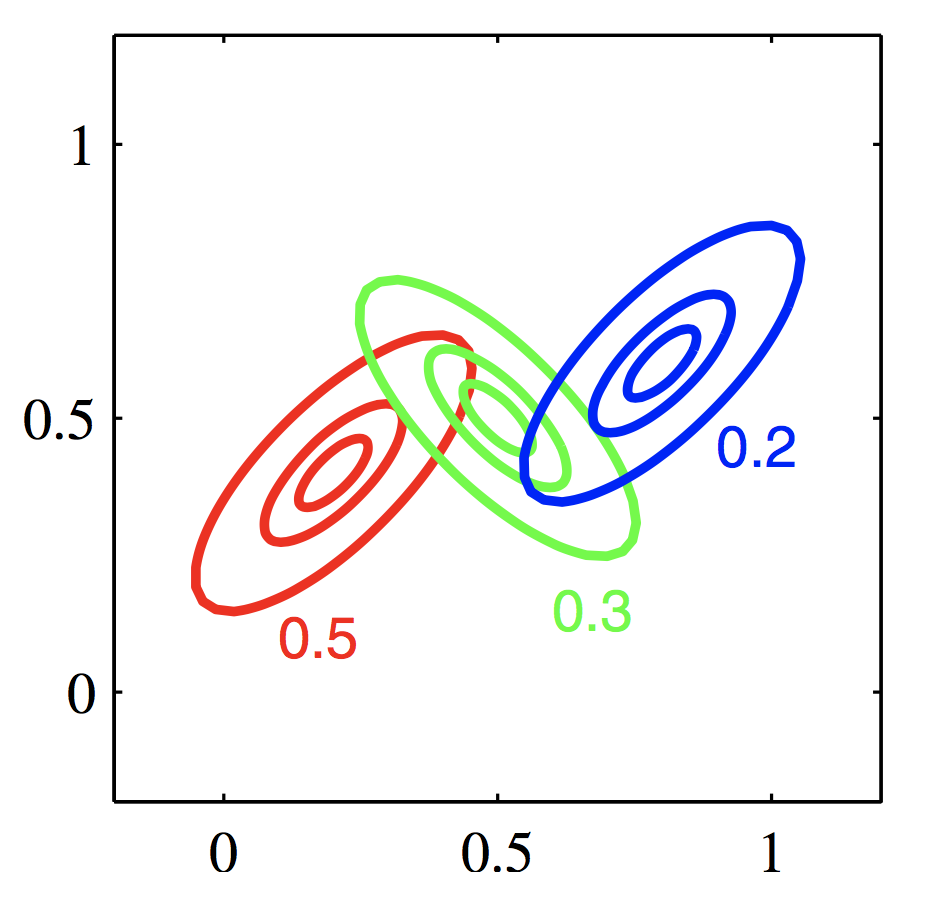
\includegraphics[width=0.75\linewidth]{figs/mixture_of_gaussians}
			\end{figure}
			\vspace{-0.5cm}
			\begin{itemize}
				\item $p(\bx | z, \btheta) = \cN(\bmu_z, \bSigma_z)$
				\item $p(z) = \Cat(\bpi)$
			\end{itemize}
		\end{minipage}%
        \eqpause
		\begin{minipage}[t]{0.53\columnwidth}
			\textit{PCA Model} \\
			\vspace{-0.5cm}
			\begin{figure}
				\centering
				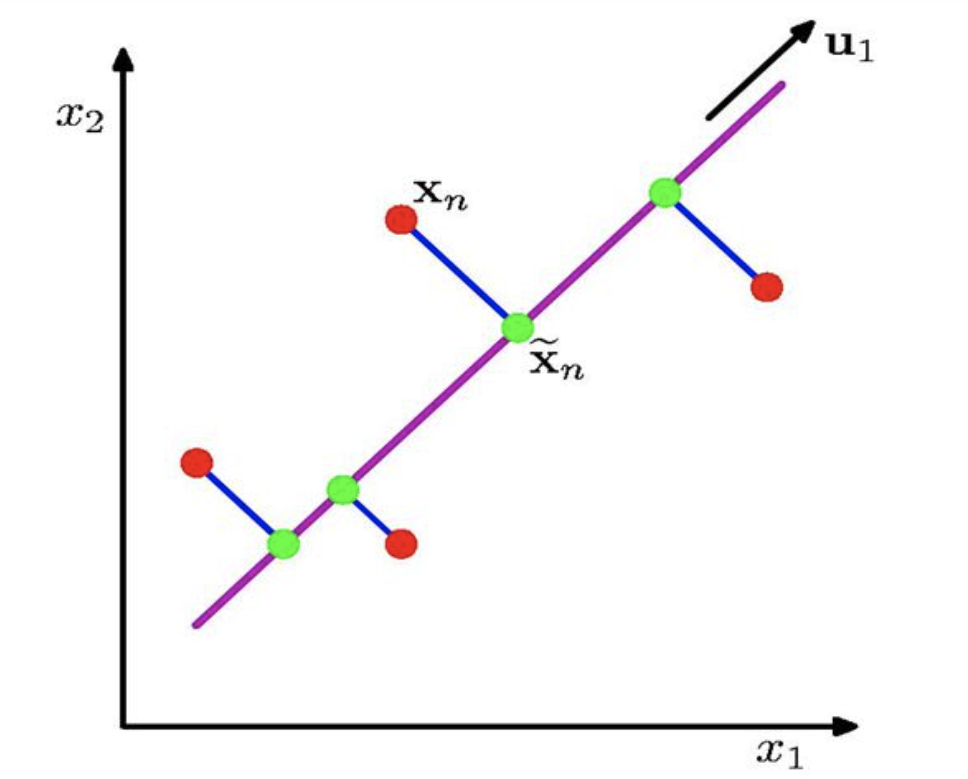
\includegraphics[width=.7\linewidth]{figs/pca}
			\end{figure}
			\vspace{-0.3cm}
			\begin{itemize}
				\item $p(\bx | \bz, \btheta) = \cN(\bW \bz + \bmu, \sigma^2 \bI)$
				\item $p(\bz) = \cN(0, \bI)$
			\end{itemize}
		\end{minipage}
	\end{block}
\end{frame}
%=======
\begin{frame}{MLE for LVM}
    \myfootnotewithlink{https://jmtomczak.github.io/blog/4/4\_VAE.html}{image credit: https://jmtomczak.github.io/blog/4/4\_VAE.html}
	\[
		\sum_{i=1}^n \log p(\bx_i | \btheta) = \sum_{i=1}^n \log \int p(\bx_i| \bz_i, \btheta) p(\bz_i) d\bz_i \rightarrow \max_{\btheta}.
	\]
    \eqpause
	\vspace{-0.7cm}
	\begin{figure}
		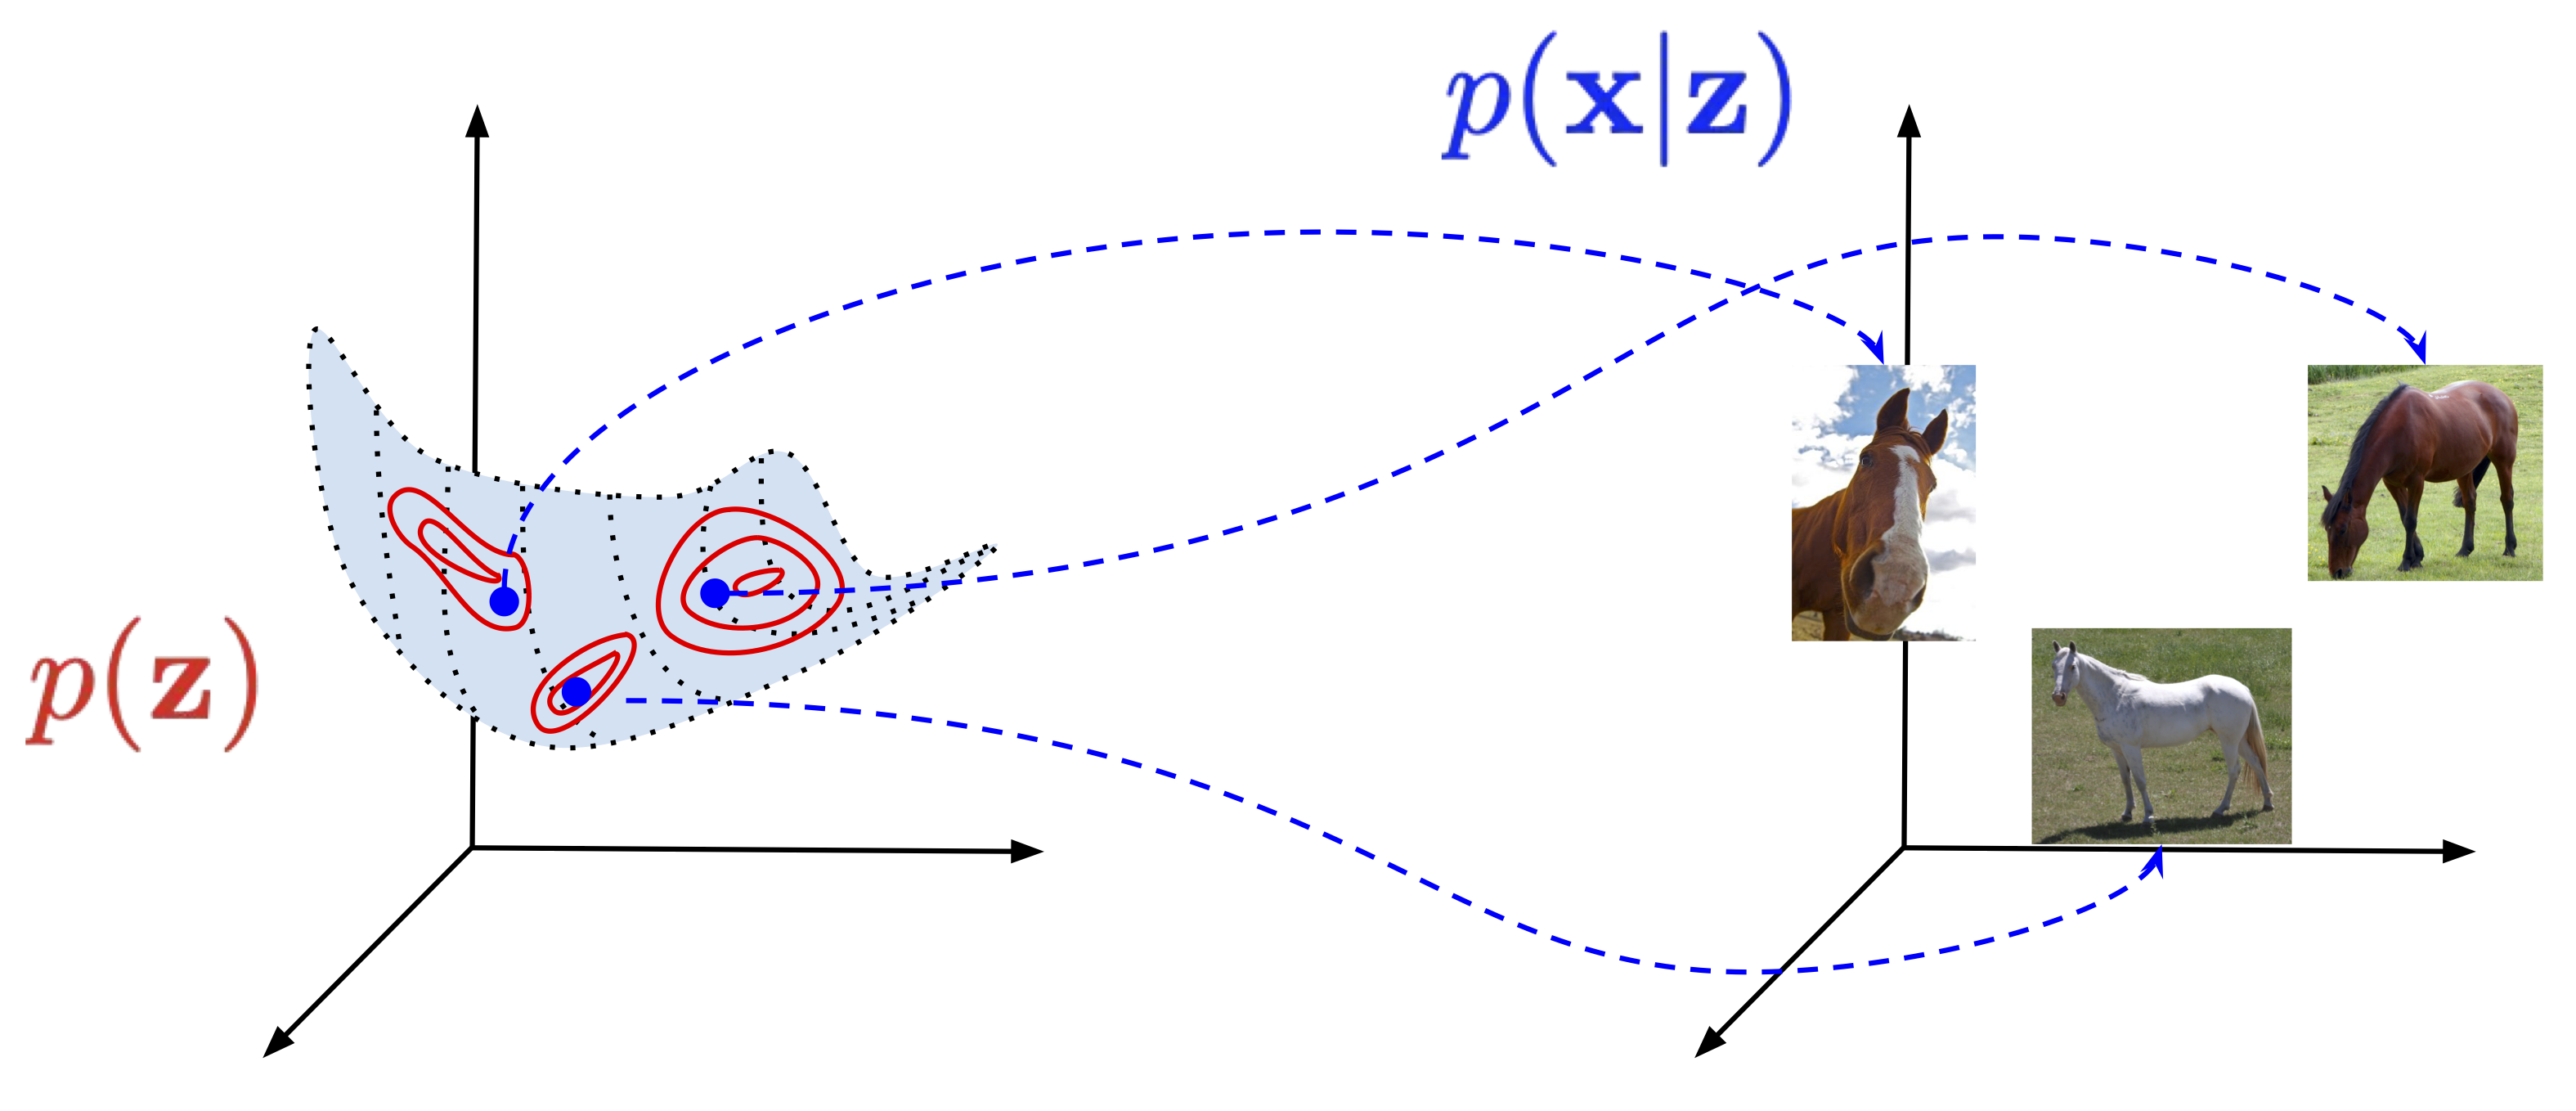
\includegraphics[width=.65\linewidth]{figs/lvm_diagram}
	\end{figure}
    \eqpause
	\vspace{-0.5cm}
	\begin{block}{Naive Approach}
		\vspace{-0.7cm}
		\[
			p(\bx | \btheta) = \int p(\bx | \bz, \btheta) p(\bz) d\bz = \bbE_{p(\bz)} p(\bx | \bz, \btheta) \approx \frac{1}{K} \sum_{k=1}^{K} p(\bx | \bz_k, \btheta),
		\]
		\vspace{-0.5cm} \\
		where $\bz_k \sim p(\bz)$. \\
        \eqpause
		\textbf{Challenge:} As the dimensionality of $\bz$ increases, the number of samples needed to adequately cover the latent space grows exponentially.
	\end{block}
\end{frame}
%=======
\section{Variational Evidence Lower Bound (ELBO)}
%=======
\begin{frame}{ELBO Derivation I}
	\begin{block}{Inequality Derivation}
		\vspace{-0.7cm}
		\begin{multline*}
			\log p(\bx| \btheta) 
			= \log \int p(\bx, \bz | \btheta) d\bz 
			\nextonslide{= \log \int \frac{q(\bz)}{q(\bz)} p(\bx, \bz | \btheta) d\bz}
			\nextonslide{= \\ = \log \bbE_{q} \left[\frac{p(\bx, \bz| \btheta)}{q(\bz)} \right]}
			\nextonslide{ \geq \bbE_{q} \log \frac{p(\bx, \bz| \btheta)}{q(\bz)} = \cL_{q, \btheta}(\bx)}
		\end{multline*}
		\vspace{-0.3cm}
	\end{block}
    \eqpause
	Here, $q(\bz)$ is any distribution such that $\int q(\bz) d\bz = 1$.
    \eqpause
	\begin{block}{Variational Evidence Lower Bound (ELBO)}
		\[
			 \cL_{q, \btheta}(\bx) = \bbE_{q} \log \frac{p(\bx, \bz| \btheta)}{q(\bz)}  \leq \log p(\bx| \btheta) 
		\]
    	\eqpause
		This inequality holds for any choice of $q(\bz)$.
	\end{block}
\end{frame}
%=======
\begin{frame}{ELBO Derivation II}
	\vspace{-0.3cm}
	\[
		{\color{teal}p(\bz|\bx, \btheta) = \frac{p(\bx, \bz | \btheta)}{p(\bx| \btheta)}}
	\]
	\vspace{-0.4cm}
	\begin{block}{Equality Derivation}
		\vspace{-0.7cm}
		\begin{multline*}
			\cL_{q, \btheta}(\bx) = \int q(\bz) \log \frac{\color{teal}p(\bx, \bz | \btheta)}{q(\bz)}d\bz 
			\nextonslide{= \\ = \int q(\bz) \log \frac{\color{teal}p(\bz|\bx, \btheta)p(\bx| \btheta)}{q(\bz)}d\bz}
			\nextonslide{ = \\ = \int q(\bz) \log p(\bx| \btheta) d\bz + \int q(\bz) \log \frac{p(\bz|\bx, \btheta)}{q(\bz)}d\bz}
			\nextonslide{ = \\ = \log p(\bx| \btheta) - \KL(q(\bz) \| p(\bz|\bx, \btheta))}
		\end{multline*}
	\end{block}
    \eqpause
	\vspace{-0.7cm}
	\begin{block}{Variational Decomposition}
		\vspace{-0.2cm}
		\[
			\log p(\bx| \btheta) = \cL_{q, \btheta}(\bx) + {\color{violet}\KL(q(\bz) \| p(\bz|\bx, \btheta))} \geq \cL_{q, \btheta}(\bx).
		\]
	\end{block}
    \eqpause
	Here, ${\color{violet}\KL(q(\bz) \| p(\bz|\bx, \btheta)) \geq 0}$.
\end{frame}
%=======
\begin{frame}{Variational Evidence Lower Bound (ELBO)}
	\vspace{-0.3cm}
	\begin{align*}
		\cL_{q, \btheta}(\bx) &= \int q(\bz) \log \frac{\color{violet}p(\bx, \bz | \btheta)}{\color{teal}q(\bz)}d\bz \\ 
		\nextonslide{&= \int q(\bz) \log {\color{violet}p(\bx | \bz, \btheta)} d\bz + \int q(\bz) \log \frac{\color{violet}p(\bz)}{\color{teal}q(\bz)}d\bz} \\ 
		\nextonslide{&= \bbE_{q} \log p(\bx | \bz, \btheta) - \KL (q(\bz) \| p(\bz))}
	\end{align*}
    \eqpause
	\vspace{-0.5cm}
	\begin{block}{Log-Likelihood Decomposition}
		\vspace{-0.8cm}
		\begin{multline*}
			\log p(\bx| \btheta) = {\color{olive}\cL_{q, \btheta}(\bx)} + \KL(q(\bz) \| p(\bz|\bx, \btheta)) 
			\nextonslide{ = \\ = {\color{olive}\bbE_{q} \log p(\bx | \bz, \btheta) - \KL (q(\bz) \| p(\bz))} + \KL(q(\bz) \| p(\bz|\bx, \btheta)).}
		\end{multline*}
		\vspace{-0.7cm}
	\end{block}
    \eqpause
	\begin{itemize}
		\item Instead of maximizing the likelihood, maximize the ELBO:
		\[
		\max_{\btheta} p(\bx | \btheta) \quad \rightarrow \quad \max_{q, \btheta} \cL_{q, \btheta}(\bx)
		\]
        \eqpause
		\vspace{-0.3cm}
		\item Maximizing the ELBO with respect to the \textbf{variational} distribution $q$ is equivalent to minimizing the KL divergence:
		\[
		\argmax_q \cL_{q, \btheta}(\bx) \equiv \argmin_q \KL(q(\bz) \| p(\bz|\bx, \btheta)).
		\]
	\end{itemize}
\end{frame}
%=======
\section{EM-Algorithm}
%=======
\begin{frame}{EM-Algorithm}
	\vspace{-0.5cm}
	\begin{multline*}
		\cL_{q, \btheta}(\bx)  =  \bbE_{q} \log p(\bx | \bz, \btheta) - \KL (q(\bz) \| p(\bz)) = \\ = \bbE_q \Big[ \log p(\bx | \bz, \btheta) - \log \frac{q(\bz)}{p(\bz)} \Big]d\bz \rightarrow \max_{q, \btheta}.
	\end{multline*}
    \eqpause
	\vspace{-0.5cm}
	\begin{block}{Block-Coordinate Optimization}
		\begin{itemize}
			\item Initialize $\btheta^*$;
            \eqpause
			\item \textbf{E-step} (optimize $\cL_{q, \btheta}(\bx)$ over $q$):
			\vspace{-0.5cm}
			\begin{multline*}
				q^*(\bz) = \argmax_q \cL_{q, \btheta^*}(\bx) = \\
				= \argmin_q \KL(q(\bz) \| p(\bz | \bx, \btheta^*)) = p(\bz| \bx, \btheta^*);
			\end{multline*}
            \eqpause
			\vspace{-0.3cm}
			\item \textbf{M-step} (optimize $\cL_{q, \btheta}(\bx)$ over $\btheta$):
			\vspace{-0.2cm}
			\[
				\btheta^* = \argmax_{\btheta} \cL_{q^*, \btheta}(\bx);
			\]
			\vspace{-0.3cm}
            \eqpause
			\item Repeat the E-step and M-step until convergence.
		\end{itemize}
	\end{block}
\end{frame}
%=======
\begin{frame}{EM-Algorithm Illustration}
    \myfootnote{Bishop\,C. Pattern Recognition and Machine Learning, 2006}
	\begin{minipage}[t]{0.45\columnwidth}
		\begin{figure}
			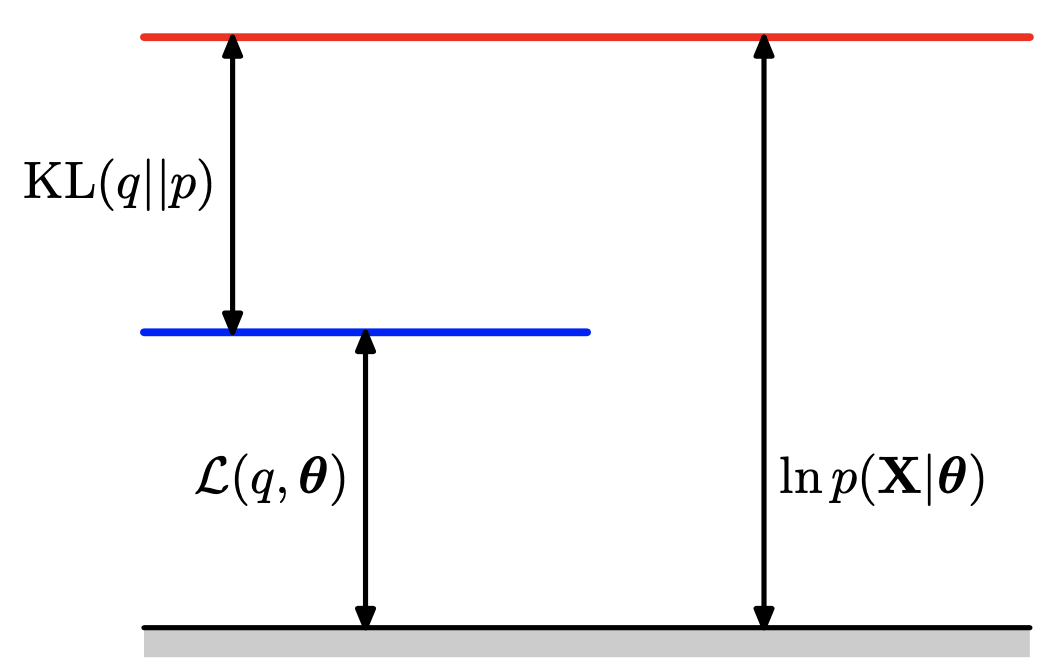
\includegraphics[width=0.9\linewidth]{figs/em_bishop1}
		\end{figure}
	\end{minipage}%
	\begin{minipage}[t]{0.55\columnwidth}
		\begin{figure}
			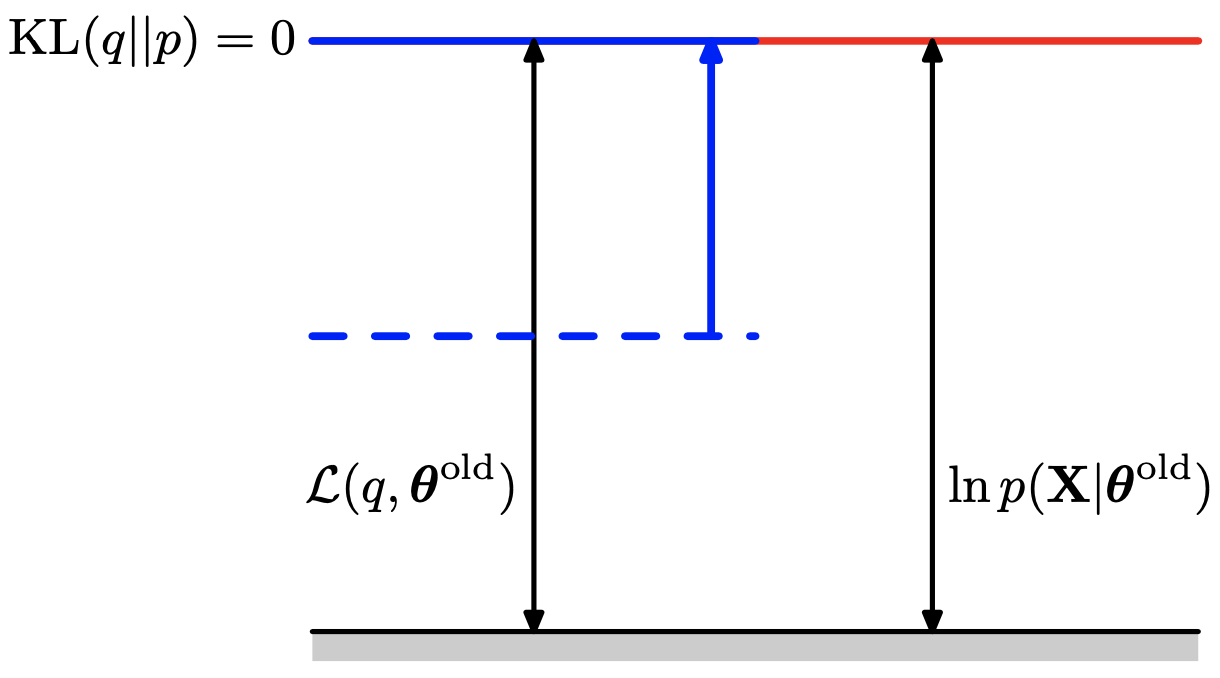
\includegraphics[width=0.85\linewidth]{figs/em_bishop2}
		\end{figure}
	\end{minipage}
    \eqpause
	\begin{figure}
		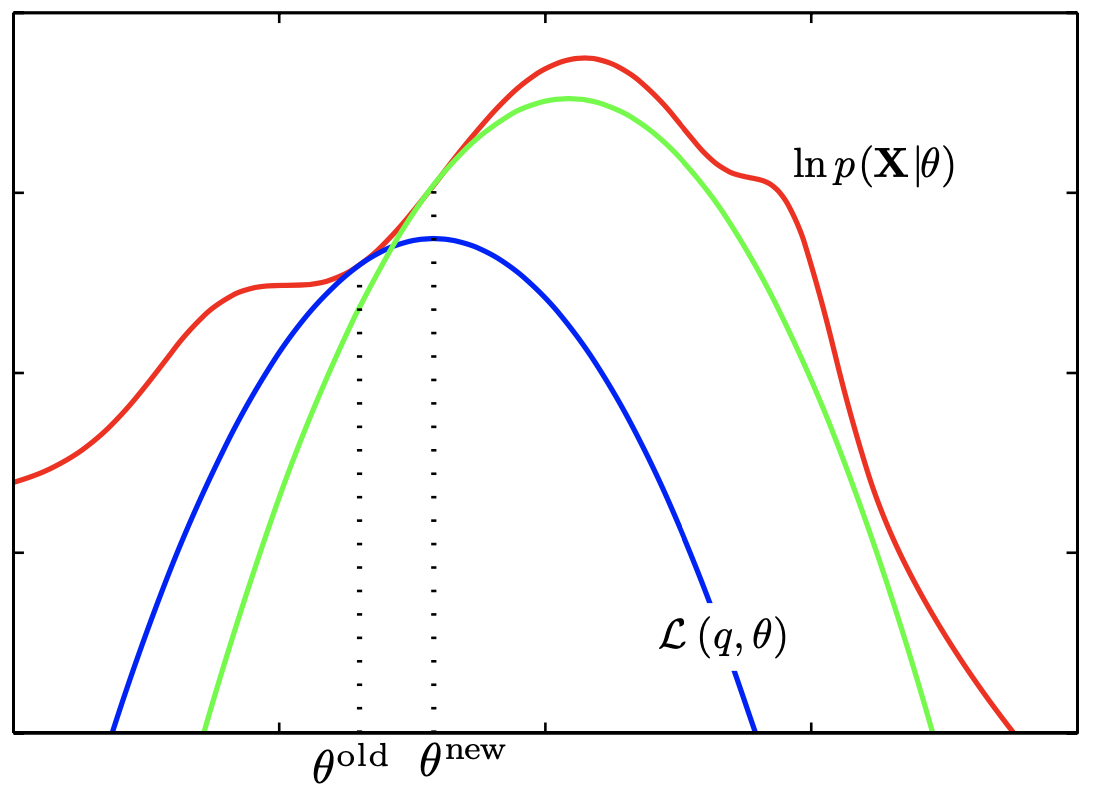
\includegraphics[width=.55\linewidth]{figs/em_bishop3}
	\end{figure}
\end{frame}
%=======
\section{Amortized Inference}
%=======
\begin{frame}{Amortized Variational Inference}
	\begin{block}{E-step}
		\vspace{-0.3cm}
		\[
			q(\bz) = \argmax_q \cL_{q, \btheta^*}(\bx) = \argmin_q \KL(q \| p) =
		p(\bz| \bx, \btheta^*).
		\]
		\eqpause
		$q(\bz)$ approximates the true posterior $p(\bz| \bx, \btheta^*)$, hence it is called \textbf{variational posterior}.				
		\eqpause
		\begin{itemize}
			\item {\color{violet}$p(\bz| \bx, \btheta^*)$ may be \textbf{intractable}};
			\item {\color{teal}$q(\bz)$ is individual for each data point $\bx$}.
		\end{itemize}
	\end{block}
	\eqpause
	\begin{block}{Variational Bayes}
		We restrict the family of possible distributions $q(\bz)$ to a parametric class $q(\bz|\bx, \bphi)$, {\color{teal}conditioned on data $\bx$} and {\color{violet}parameterized by $\bphi$}.
		\eqpause
		\begin{itemize}
			\item E-step
			\[
				\bphi_k = \bphi_{k-1} + \left.\eta \cdot \nabla_{\bphi} \cL_{\bphi, \btheta_{k-1}}(\bx)\right|_{\bphi=\bphi_{k-1}}
			\]
			\item M-step
			\[
				\btheta_k = \btheta_{k-1} + \left.\eta \cdot \nabla_{\btheta} \cL_{\bphi_k, \btheta}(\bx)\right|_{\btheta=\btheta_{k-1}}
			\]
		\end{itemize}
	\end{block}
\end{frame}
%=======
\begin{frame}{Variational EM Illustration}
	\myfootnote{Bishop C., Deep Learning: Foundations and Concepts, 2024}
	\begin{itemize}
		\item E-step:
		\[
			\bphi_k = \bphi_{k-1} + \left.\eta \cdot \nabla_{\bphi} \cL_{\bphi, \btheta_{k-1}}(\bx)\right|_{\bphi=\bphi_{k-1}}
		\]
		\item M-step:
		\[
			\btheta_k = \btheta_{k-1} + \left.\eta \cdot \nabla_{\btheta} \cL_{\bphi_k, \btheta}(\bx)\right|_{\btheta=\btheta_{k-1}}
		\]
	\end{itemize}
	\begin{figure}
		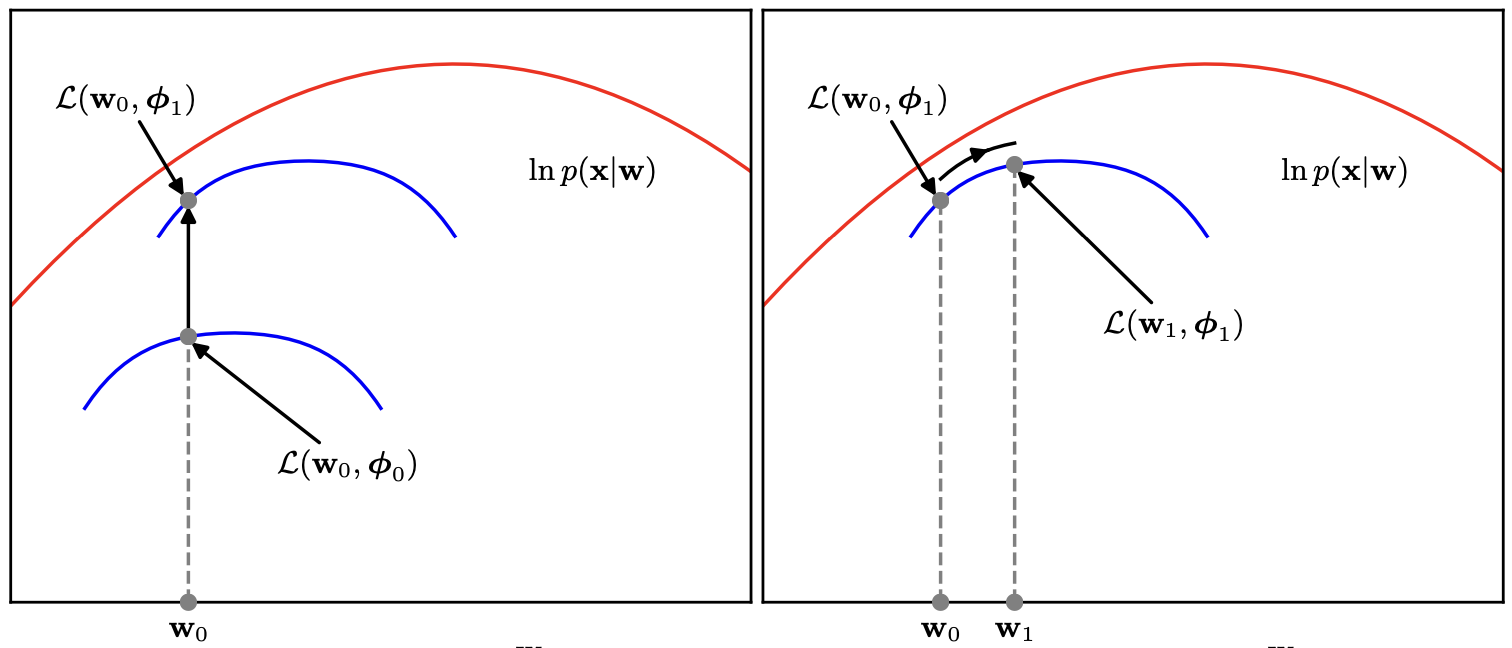
\includegraphics[width=\linewidth]{figs/em_bishop4}
	\end{figure}
		
\end{frame}
%=======
\begin{frame}{Variational EM Algorithm}
	\begin{block}{ELBO}
		\vspace{-0.5cm}
		\[
			\log p(\bx| \btheta) = \cL_{\bphi, \btheta}(\bx) + \KL(q(\bz | \bx, \bphi) \| p(\bz|\bx, \btheta)) \geq \cL_{\bphi, \btheta}(\bx).
		\]
		\[
		 	\cL_{q, \btheta}(\bx) = \bbE_{q} \log p(\bx | \bz, \btheta) - \KL(q(\bz | \bx, \bphi) \| p(\bz))
		\]
		\vspace{-0.5cm}
	\end{block}
	\eqpause
	\begin{itemize}
		\item \textbf{E-step:}
		\vspace{-0.3cm}
		\[
			\bphi_k = \bphi_{k-1} + \left.\eta \cdot \nabla_{\bphi} \cL_{\bphi, \btheta_{k-1}}(\bx)\right|_{\bphi=\bphi_{k-1}},
		\]
		\vspace{-0.3cm} \\
		where $\bphi$ denotes the parameters of the variational posterior $q(\bz | \bx, \bphi)$.
		\item \textbf{M-step:}
		\[
			\btheta_k = \btheta_{k-1} + \left.\eta \cdot \nabla_{\btheta} \cL_{\bphi_k, \btheta}(\bx)\right|_{\btheta=\btheta_{k-1}},
		\]
		where $\btheta$ represents the parameters of the generative model $p(\bx | \bz, \btheta)$.
	\end{itemize}
	\eqpause
	The remaining step is to obtain \textbf{unbiased} Monte Carlo estimates of the gradients: $\nabla_{\bphi} \cL_{\bphi, \btheta}(\bx)$ and $\nabla_{\btheta} \cL_{\bphi, \btheta}(\bx)$. 
\end{frame}
%=======
\begin{frame}{Summary}
	\begin{itemize}
		\item The Bayesian framework generalizes nearly all standard machine learning methods.
		\vfill
		\item LVMs introduce latent representations for observed data, enabling more interpretable models.
		\vfill
		\item LVMs maximize the variational evidence lower bound (ELBO) to obtain maximum likelihood estimates for the parameters.
		\vfill
		\item The general variational EM algorithm optimizes the ELBO within LVMs to recover the MLE for the parameters $\btheta$.
		\vfill
		\item Amortized variational inference enables efficient estimation of the ELBO via Monte Carlo estimation.
	\end{itemize}
\end{frame}
\end{document}